%% LyX 2.3.4.2 created this file.  For more info, see http://www.lyx.org/.
%% Do not edit unless you really know what you are doing.
\documentclass[english]{article}
\usepackage[T1]{fontenc}
\usepackage[latin9]{inputenc}
\usepackage{amsmath}
\usepackage{amsthm}
\usepackage{amssymb}
\usepackage{graphicx}

\makeatletter

%%%%%%%%%%%%%%%%%%%%%%%%%%%%%% LyX specific LaTeX commands.
%% Because html converters don't know tabularnewline
\providecommand{\tabularnewline}{\\}

%%%%%%%%%%%%%%%%%%%%%%%%%%%%%% Textclass specific LaTeX commands.
\theoremstyle{plain}
\newtheorem{thm}{\protect\theoremname}
\theoremstyle{remark}
\newtheorem{rem}[thm]{\protect\remarkname}
\theoremstyle{plain}
\newtheorem{prop}[thm]{\protect\propositionname}
\theoremstyle{definition}
\newtheorem{example}[thm]{\protect\examplename}

\makeatother

\usepackage{babel}
\providecommand{\examplename}{Example}
\providecommand{\propositionname}{Proposition}
\providecommand{\remarkname}{Remark}
\providecommand{\theoremname}{Theorem}

\begin{document}
\global\long\def\G{\mathcal{G}}%
\global\long\def\F{\mathcal{F}}%
\global\long\def\var{\mathcal{\mathrm{var}}}%
\global\long\def\E{\mathbb{E}}%
\global\long\def\defined{\stackrel{\text{def}}{=}}%
\global\long\def\Bi{\mathcal{\mathrm{Bi}}}%
\global\long\def\indep#1{{\perp\hspace{-2mm}\perp}#1}%
\global\long\def\P{\mathbb{P}}%
\global\long\def\N{\mathbb{N}}%
\global\long\def\U{\mathbb{U}}%
\global\long\def\E{\mathbb{E}}%
\global\long\def\R{\mathbb{R}}%
\global\long\def\G{\mathcal{G}}%
\global\long\def\g{\mathbb{\Pi}}%
\global\long\def\F{\mathcal{F}}%
\global\long\def\S{\mathcal{S}}%
\global\long\def\Q{\mathcal{Q}}%
\global\long\def\B{\mathcal{B}}%
\global\long\def\ND{\mathcal{N}}%
\global\long\def\XX{\mathcal{X}}%
\global\long\def\indep#1{{\perp\hspace{-2mm}\perp}#1}%
\global\long\def\L{\mathcal{L}}%
\global\long\def\var{\mathrm{var}}%
\global\long\def\cov{\mathrm{cov}}%
\global\long\def\charf{\mathbf{1}}%
\global\long\def\d{\mathrm{d}}%
\global\long\def\M{\mathcal{M}}%
\global\long\def\T{\mathcal{T}}%
\global\long\def\Exp{\mathrm{Exp}}%
\global\long\def\Uniform{\mathrm{U}}%
\global\long\def\eqd{{d\atop =}}%
\global\long\def\A{\mathcal{A}}%
\global\long\def\I{\mathcal{I}}%
\global\long\def\X{\mathcal{X}}%
\global\long\def\supp{\mathrm{support}}%
\global\long\def\H{\mathcal{H}}%
\global\long\def\Z{\mathcal{Z}}%
\global\long\def\as{\qquad a.s.}%
\global\long\def\on{\qquad\text{on }}%
\global\long\def\C{\mathcal{C}}%
\global\long\def\barxi{\overline{\xi}}%
\global\long\def\Po{\mathrm{Po}}%
\global\long\def\barvs{\overline{\varsigma}}%
\global\long\def\bareps{\overline{\varepsilon}}%
\global\long\def\bari{\overline{\iota}}%
\global\long\def\barx{\overline{x}}%
\global\long\def\baru{\overline{u}}%
\global\long\def\bars{\overline{s}}%
\global\long\def\Bi{\mathrm{Bi}}%
\global\long\def\defined{\stackrel{\text{def }}{=}}%
\global\long\def\d{\mathbf{d}}%
\global\long\def\dw{\mathrm{d}}%
\global\long\def\bary{\overline{y}}%
\global\long\def\cvar{\mathrm{CVaR}}%
\global\long\def\barP{P}%
\global\long\def\barX{\overline{X}}%
\global\long\def\barP{\overline{P}}%
\global\long\def\barT{\overline{T}}%
\global\long\def\barB{\overline{B}}%
\global\long\def\barI{\overline{I}}%

\title{SEIR Filter -- Stochastic Model of Pandemics}
\author{Martin �m�d, Lud\v{e}k Berec, Ale� Anton�n Kub\v{e}na, Jan Trnka,
V�t Tu\v{c}ek, Milan Zaj�\v{c}ek,}
\maketitle

\section{Introduction}

To cope with the present pandemic, there are lots of epidemiological
models at hand. Most of them are working well, simply because is not
difficult to fit (nearly) exponential growth/decline and it is not
difficult to make the growth factor dependent on various covariates.
What is difficult, however, is to distinguish the impact of the factors
from random fluctuations. Moreover, as many counter-measures as well
as their release come hand in hand, it is hard to distinguish their
impact. In statistics, the former phenomenon is called insignificance,
the latter either non-idetifiability (if the data do not allow to
distinguish two parameters) or co-linearity (if the parameters cannot
be distinguished with sufficient certainty). Last but not least, the
epidemics is observed only indirectly through incomplete data. Needless
to say that, once these phenomenons are not taken into account or
are handled insufficiently, wrong policy recommendations stem from
the models.

Mathematical statistics disposes of tools to handle all significance,
co-linearity and partial observability; however, to our best knowledge,
there is no work systematically doing so for compartment epidemiological
models. The goal of the present paper is to start filling this gap
by proposing a general stochastic epidemiological model, which we
call SEIR Filter.

Our model is a discrete time discrete space one. Next we argue that
this is the best choice for practical use.

There is a large literature on continuous time diffusion epidemiological
models, see e.g. \cite{farnoosh2017stochastic} and the references
therein. Yet these models are able to capture global properties of
an epidemics and handle noise, their practical usage is limited as
it is difficult to incorporate heterogeneity, caused by non-pharmaceutical
interventions, into these models. Moreover, given discrete time data,
discretizations of these models is needed which do not inherit their
favorable properties.

Another wide class of models are those with continuous time and discrete
state space. In \cite{gibson1998estimating}, for instance, such model
together with an estimation procedure is developed. Yet these models
are realistic, respecting integer sizes of the compartments, again
there is a problem with their application in practice due to discrete
nature of observed data.

As we have premised, we regard discrete-time discrete-space stochastic
models as the most practical. One of the models closest to our one
is that by \cite{kucharski2020early} (or \cite{prem2020effect}).
When estimating its parameters, the authors use Monte Carlo simulation
to evaluate likelihood functions. We argue and demonstrate that the
parameters of these models can be estimated more straightforward way,
as the likelihood (or other estimating) function can be computed exactly,
allowing for quicker and more reliable estimation.

In addition to the tractability of the estimating functions, our model
allows for closed form formulas for expected future compartment sizes
and for reproduction number. We also give simple criteria for vanishing
and explosion of the epidemics, as well as bounds of limiting expected
sizes given stationary imports. All this allows various applications
of the model, e.g. in optimal control of the pandemics, which we also
demonstrate.

After a rigorous probabilistic formulation of the model (Section \ref{sec:Model-Definition}),
we discuss its basic probabilistic properties (Section \ref{sec:Model-Properties}),
its autonomous sub-models and reproduction number (Section \ref{sec:Sub-models-and-Replication})
and asymptotic properties (Section \ref{sec:Asymptotic-behavior}).
Next, we introduce an age-cohort version of the model (Section \ref{sec:cohorts})
and suggest a way of optimal control of the epidemics (Section \ref{sec:oc}).
Further, we discuss estimation of the model (Section \ref{sec:Estimation}).
Next, apply our model to the COVID pandemics in Czech Republic 2020
(Section \ref{sec:Application-to-The}) and demonstrate its possible
applications by the comparison of three vaccination scenarios (Section
\ref{sec:Vaccination-Experiment}). Finally, we conclude the paper
(Section \ref{sec:Conclusion}).

\section{Model Definition}

\label{sec:Model-Definition}Assume a population of size $s\in\N$,
where $s$ is large. Each individual of the population is either susceptible,
or finds himself in one of the compartments $S_{1},\dots,S_{k}$.
Let $I_{t}\in\N_{0}^{k},$ $t\in\N_{0}^{+},$ be a possibly hidden
external inflow (import) of individuals into the compartments and
let $Z_{t}\in\R^{p},$ $t\in\N_{0}^{+}$, be an observed exogenous
process.

For any $t\in\N_{0}$, let $X_{t}=(X_{t}^{1},\dots,X_{t}^{k})\in\N_{0}^{k},t\in\N_{0},$
be a possibly hidden stochastic process of the compartment sizes which
we define later. Let 
\[
Y_{t}\in\R^{n},\qquad Y_{t}=FX_{t}+\epsilon_{t},\qquad t\in\N_{0},
\]
be a process of observations where $F$ is a deterministic $n\times k$
matrix with rank $n$, and $\epsilon_{t}$ is a random errors vector. 

Denote $(\F_{t})_{t\geq0}$ and $(\G_{t})_{t\geq0}$ the filtrations
induced by $(X,Y,I,Z)$, by $(Y,Z)$, respectively -- these filtrations
may be seen as information flows, $(\F_{t})$ representing all the
information and $(\G_{t})$ the observable one. 

We assume that 
\[
\E(\epsilon_{t+1}|\F_{t})=0,\qquad\var(\epsilon_{t+1}|\F_{t})=\mathrm{diag(}\Gamma_{t}(X_{t},X_{t}^{2})),\qquad t\in\N_{0},
\]
where $\Gamma_{t}$ is a $\G_{t}$-measurable affine linear function
(i.e. $\Gamma_{t}(x,y)=\gamma_{t,0}+\gamma_{t,1}x+\gamma_{t,2}y$
for some $\gamma_{t,0}\in\R^{k}$ and $\gamma_{t,1},\gamma_{t,2}\in\R^{k\times k}$
where all $\gamma_{t,0},\gamma_{t,1}$ and $\gamma_{t,2}$ are $\G_{t}$-measurable). 

We define $X$ recursively: We let $X_{0}$ to be a possibly random
vector and, for any $t\in\N$, we put 
\[
X_{t+1}=I_{t}+N_{t+1}+M_{1,t+1}+\dots+M_{k,t+1}.
\]
Here, $N_{t+1}\in\N_{0}^{k}$ is the inflow of domestically infected
individuals such that $N_{t+1}|\F_{t}\text{\ensuremath{\sim\mathrm{C\Po}(A_{t}X_{t},L)}}$
where $A_{t}=(\alpha_{t}^{ij})_{1\leq i,j\leq k}$, $A_{t}\in\G_{t}$
is a random matrix (the notation $A_{t}\in\G_{t}$ means that $A_{t}$
is a $(\G_{t})$-adapted process) and, for any vector $x$, $\mathrm{CPo}(x,L)$
stands for a vector of independent Compound Poisson variables with
the intensities given by $x$ and the embedded distribution $L$.
Observe that, by basic properties of Compound Poisson distribution,
\[
\frac{\var(N_{t+1}^{i}|\F_{t})}{\E(N_{t+1}^{i}|\F_{t})}=v\defined\frac{\E L^{2}}{\E L}
\]
 (with $\frac{0}{0}\defined\frac{\E L^{2}}{\E L})$, $t\geq0,1\leq i\leq k$.
Further, for any $i$, $M_{i,t+1}\in\N_{0}^{k}$ is the distribution\footnote{Here, we do not mean a probability distribution, but the numbers of
individuals having ended in individual compartments.} of those, who found themselves in compartment $i$ at $t$, between
the compartments at $t+1$. In particular, $M_{i,t+1}^{j}$ (the $j$-th
component of $M_{i,t+1}$) is the number of the individuals who transited
from the compartment $j$ to the compartment $i$ between $t$ to
$t+1$. Further we assume $M_{i,t+1}$, for any $i$, to follow Dirichlet
Multinomial (DM) conditional distribution with parameters $\left(X_{t}^{i},\frac{p_{t}^{1,i}}{c_{i}},\dots,\frac{p_{t}^{k,i}}{c_{i}}\right)$
where $P_{t}=(p_{t}^{ij})_{1\leq i,j\leq k}\in\G_{t}$ is a ``mean''
transition matrix and $(c_{1},\dots,c_{k})$ are deterministic dispersion
parameters. 
\begin{rem}
If we assumed the individuals to change their state according to $P_{t}$
with the transitions being conditionally independent given $\F_{t},$
then we would get $M_{i,t+1}|\F_{t}$ as Multinomial with parameters
$X_{t}^{i}$ and $P_{t}^{(i)}$ where, for any matrix $\Sigma$, $\Sigma^{(i)}$
is its $i$-th column. In practice, however, the assumption of the
conditional independence, is unrealistic, as the course of infection
differs between individuals and (due to mutations) tends to cluster.
The standard way of coping with this situation is using $\mathrm{DM}$
distribution. 
\end{rem}

The flow of individuals between states are illustrated by the following
chart.
\begin{center}
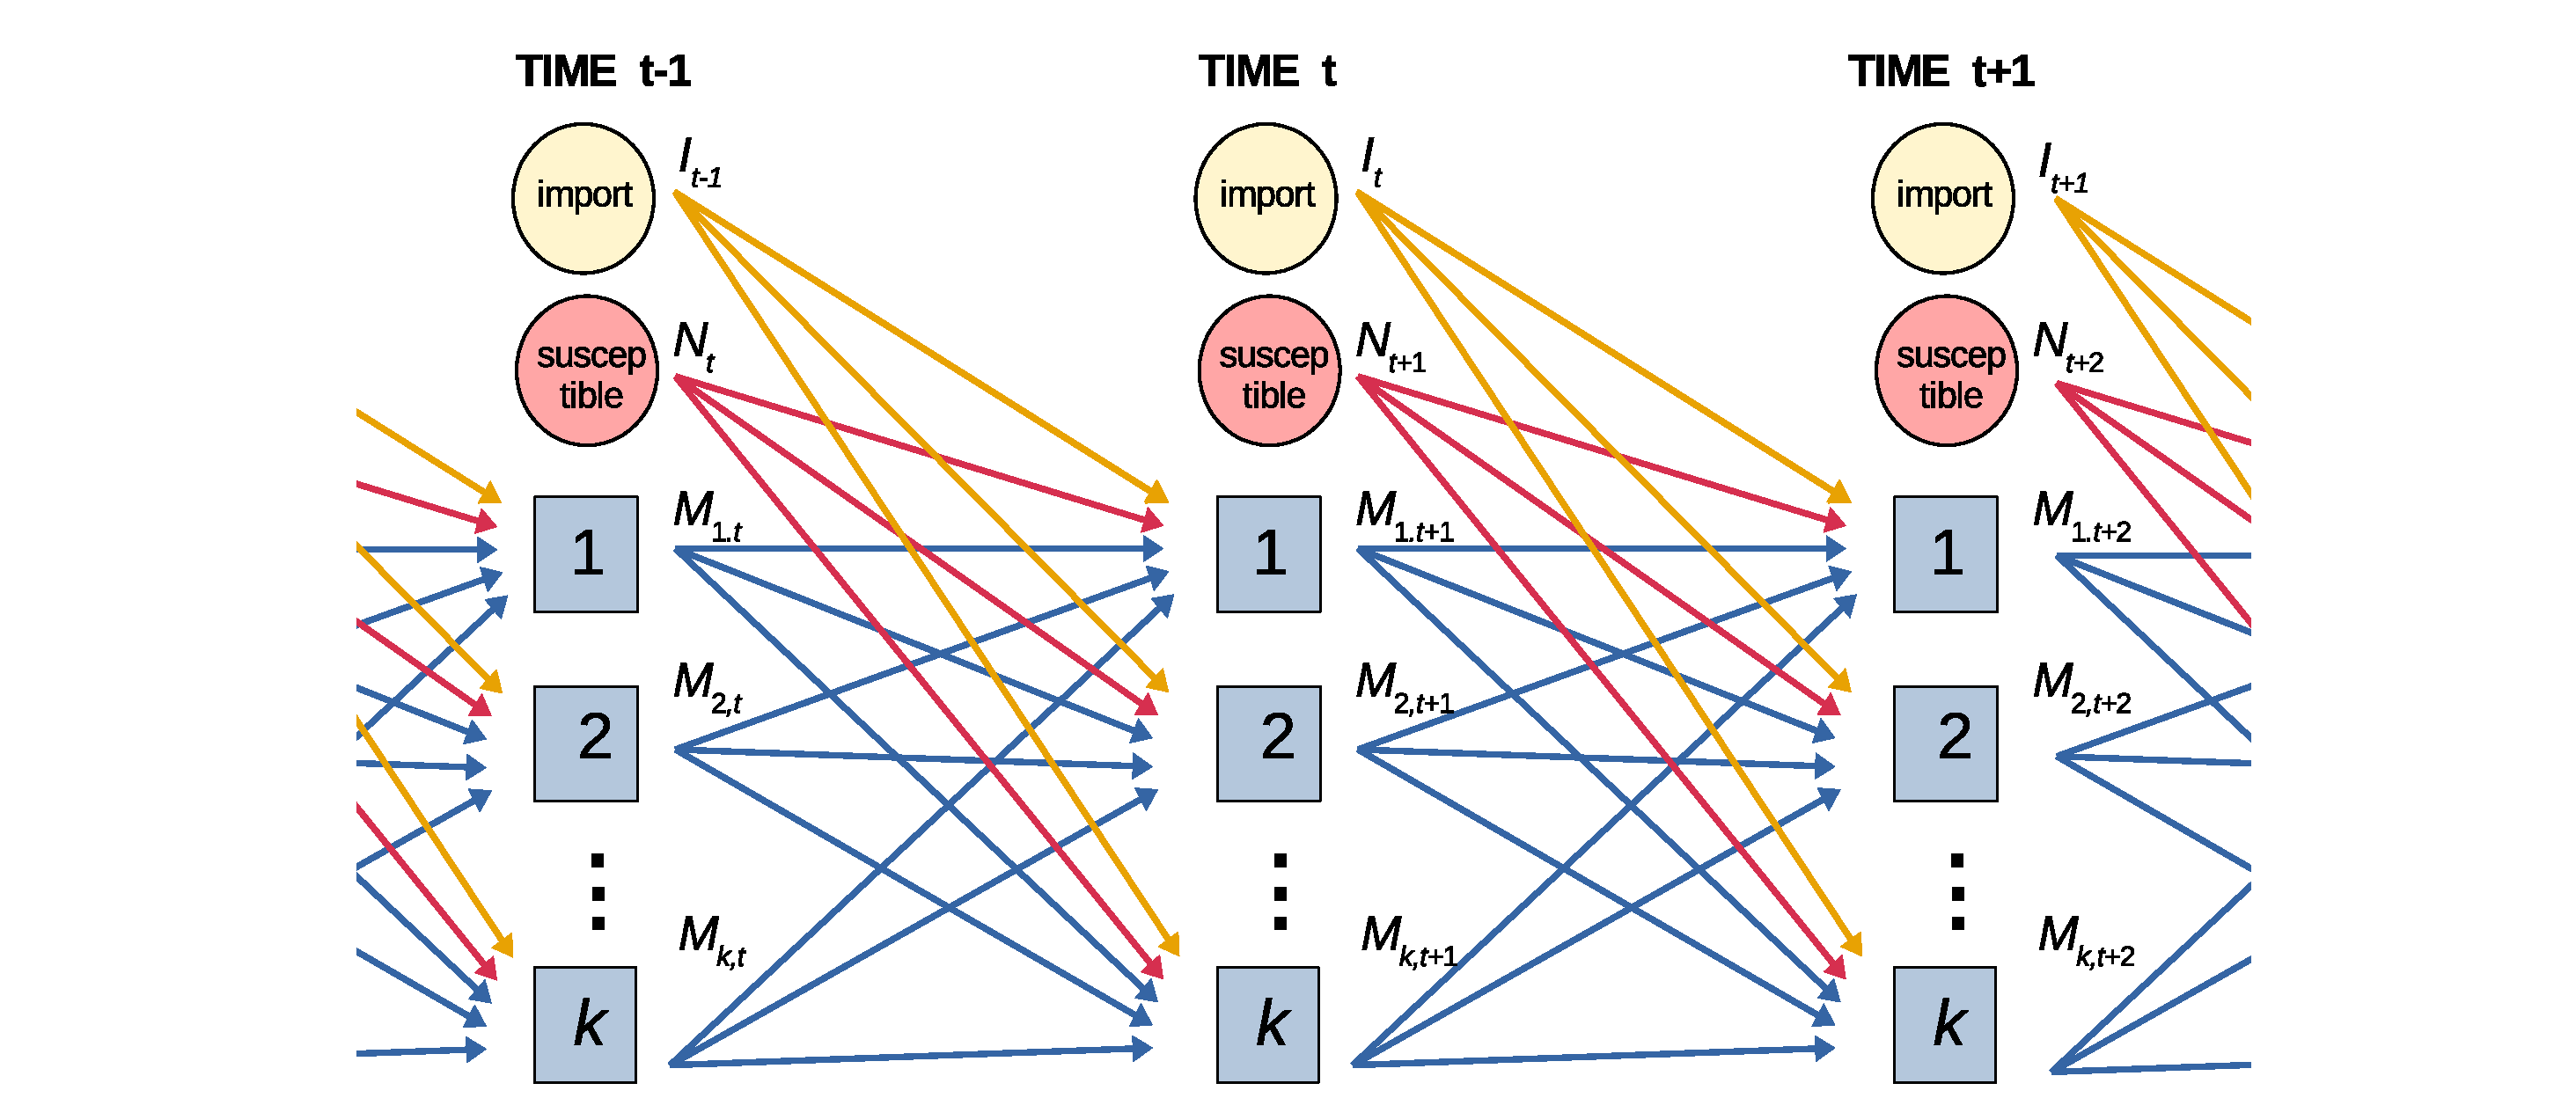
\includegraphics[scale=0.3]{schema}
\par\end{center}

Finally, we assume $N_{t+1},M_{1,t+1},\dots,M_{k,t+1},\epsilon_{t+1}$
to be mutually conditionally independent given $\F_{t}$ (which, in
words, means that all the dependence between the inflows, the transitions
and the observation can be explained by the state of the system at
$t$). Consequently,

\[
\left.X_{t+1}\right|\F_{t}\sim\bigcirc_{1\leq i\leq k}\mathrm{DM}\left(X_{t}^{i},\frac{1}{c_{i}}P_{t}^{(i)}\right)\circ\mathrm{CPo}(A_{t}X_{t},L)\circ\delta(I_{t}),
\]
where $\bigcirc$ and $\circ$ stand for the summation of (mutually)
independent random vectors.

\begin{rem}
The variability of the individual infectiousness may be naturally
reflected by the choice of $L$. To demonstrate it, assume that only
a single compartment (labeled $I$) is infectious, that all the new
infections fall to a single compartment (labeled $E$), and the number
of risk contacts of each infectious individual is Poisson. Let $t\geq0$
and denote $N_{t+1,i}$ the number of the infections, caused by the
$i$-th individual at $t$. 

If the intensity of the contact distribution and the contagion probability
were the same for all, equal to $c$, $p$, respectively, then it
would be $N_{t+1,i}\sim\Po(cq)$, $i\in\N$; consequently, $N_{t+1}^{E}\sim\Po(\lambda X_{t}^{I})$,
$\lambda=cq$, so we may put $\alpha_{t}^{EA}=\lambda$ and $L=\delta_{1}$,
having $\E(N_{t+1}^{E}|\F_{t})=\mathrm{\var}(N_{t+1}^{E}|\F_{t})=\lambda X_{t}$.

Now consider a more realistic situation in which the infectiousness
randomly varies between individuals. A standard way of modeling this
situation is assuming, for each $i$, that the intensity $\lambda_{i}$
of $N_{t+1,i}$ is chosen from Gamma distribution, implying that $N_{t+1,i}$
is negative binomial (see \cite{zhou2013negative}). In particular,
once $\lambda_{i}\sim\Gamma(k,\theta)$, and $N_{t+1,i}|\lambda_{i}=\Po(\lambda_{i})$,
we are gettomg that $N_{t+1,i}\sim\mathrm{NB}(k,p),$ $p=\frac{\theta}{1+\theta}$,
with
\begin{equation}
\E N_{t+1,i}=\kappa\defined\theta k,\qquad\var(N_{t+1,i})=\kappa v,\qquad v=1+\frac{\kappa}{k}.\label{eq:ev}
\end{equation}
As the Negative Binomial distribution can be represented by a Compound
Poisson one and as the sum of independent Compound Poisson distributions
is Compound Poisson, we have that $N_{t+1}^{E}$ is Compound Poisson\footnote{In particular, $N_{t+1,i}=\mathrm{CPo}(k\ln(1+\theta),\mathrm{Log}(p))$,
where $\mathrm{Log}$ is the Logarithmic distribution, see \cite{zhou2013negative}).
Thus, $N_{t+1}^{E}\sim\mathrm{CPo}(X_{t}^{I}k\ln(1+\theta),\mathrm{Log}(p))$
so we may put $\alpha_{t}^{EA}=k\ln(1+\theta)$, $L=\mathrm{Log}(p)$..} and it follows from (\ref{eq:ev}) that 
\[
\E(N_{t+1}^{E}|\F_{t})=\kappa X_{t},\qquad\mathrm{\var}(N_{t+1}^{E}|\F_{t})=\kappa X_{t}v
\]
\end{rem}

\begin{rem}
\label{rem:-v}\cite{endo2020estimating} claim that the total number
$T$ of persons infected by a single COVID-infectious individual is
$T\sim\mathrm{NB}($$K,P)$ where $K\doteq0.1$ and $P$ is such that
$\E T=R_{0}$ where $R_{0}$ is the basic reproduction number. As
$R_{0}$ of COVID is generally assumed to be around 2.5 and $\E T=K\frac{P}{1-P}$,
it follows that $P\doteq\frac{25}{26}$. Consequently, the variance-to-mean
ratio is $\tilde{v}\defined\frac{1}{1-P}\doteq26$. Assuming that
the individual is infectious for $f$ days and that his contacts are
restricted by a factor $\beta$, we may, in light of the Compound
Poisson reformulation of $T$, conclude that the number $N_{t+1,i}$
of daily infected is Compound Poisson with $\E N=\frac{\beta}{f}\E T,\var(N)=\frac{\beta}{f}\var(T)$,
i.e. $N_{t+1,i}$ and consequently $N_{t+1}^{E}$ has the same variance-to-mean
ratio as $T$, i.e. $v=\tilde{v}\doteq26$. 
\end{rem}

\begin{rem}
For any $x\in\N_{0},c\geq0$ and $p\in[0,1]^{k}$ such that $\sum_{i=1}^{k}p^{i}=1$,
we have 
\[
\E\left(\mathrm{DM}(x,\frac{p}{c})\right)=px=\E\left(\mathrm{Multinomial}(x,p)\right)
\]
and 
\[
\var\left(\mathrm{DM}(x,\frac{p}{c})\right)=[\mathrm{diag}(p)-pp^{T}]\frac{x+c}{1+c}x=\var(\mathrm{Multinomial}(x,p))\frac{x+c}{1+c},
\]
from which it is clear that $\mathrm{DM}(x,\frac{p}{c})\rightarrow\mathrm{Multinomial}(x,p)$
as $c\rightarrow\infty$ and that the deviation of the Multinomial
variance matrix grows with decreasing $c$.
\end{rem}


\section{Model Properties}

\label{sec:Model-Properties}By probability calculus, we get that
\begin{multline*}
\E(X_{t+1}|\F_{t})=\E(T_{t}X_{t}+I_{t}|\F_{t})=\E\left(\left.\sum_{i=1}^{k}M_{t+1,i}+N_{t+1}+I_{t}\right|\F_{t}\right)\\
\sum_{i=1}^{k}P_{t}^{(i)}X_{t}^{i}+(\E L)A_{t}X_{t}+I_{t}=T_{t}X_{t}+I_{t},
\end{multline*}
where, for any matrix $\Sigma,$ $\Sigma^{(i)}$ denotes its $i$-th
column, and 
\begin{align}
T_{t} & \defined P_{t}+B_{t},\qquad B_{t}=(\beta_{t}^{i,j})_{1\leq i,j\leq k}\defined(\E L)A_{t},\qquad t\geq0.\label{eq:t}
\end{align}
Consequently, for any $t,s\in\N_{0},t>s$, 
\begin{multline*}
\E(X_{t}|\F_{s})=\E(T_{s,t-1}X_{s}+\sum_{\theta=s}^{t-1}T_{\theta+1,t-1}I_{\theta}|\F_{s})\\
=\E(T_{s,t-1}|\F_{s})X_{s}+\sum_{\theta=s}^{t-1}\E(T_{\theta+1,t-1}I_{\theta}|\F_{s}),
\end{multline*}
where, for any matrix process $\Sigma$, $\Sigma_{s,t}\defined\Sigma_{t}\times\dots\times\Sigma_{s}$
with $\Sigma_{s,s-1}\defined E$ where $E$ is the identity matrix.

In the special case that 
\begin{equation}
B_{\tau}\equiv B_{s},\qquad P_{\tau}\equiv P_{s},\qquad s\leq\tau\leq t,\label{eq:speck}
\end{equation}
 we have 
\[
\E(X_{t}|\F_{s})=T_{s}^{t-s}X_{s}+\sum_{\tau=s}^{t-1}T_{s}^{t-\tau-1}\E(I_{\tau}|\F_{s}),
\]
and 
\[
\E(X_{t}|\G_{s})=T_{s}^{t-s}\E(X_{s}|\G_{s})+\sum_{\tau=s}^{t-1}T_{s}^{t-\tau-1}\E(I_{\theta}|\G_{s})
\]
If, in addition, $\E(I_{\theta}|\G_{s})\equiv\mu$ for some $\mu\in\G_{s}$
and $(E-T_{s})$ is invertible, the latter formula simplifies to
\[
\E(X_{t}|\G_{s})=T_{s}^{t-s}\E(X_{s}|\G_{s})+(E-T_{s})^{-1}(E-T_{s}^{t-s})\mu.
\]
As for variance, we have
\begin{multline*}
\var(X_{t+1}|\F_{t})=\sum_{i=1}^{k}\var(M_{t+1,i}|\F_{t})+\var(N_{t+1}|\F_{t})+\var(I_{t}|\F_{t})\\
=\sum_{1\leq i\leq m}\var\left(\mathrm{DM}\left(X_{t}^{i},\frac{1}{c_{i}}P_{t}^{(i)}\right)\right)+\var(\mathrm{CPo}(A_{t}X_{t},L))+0\\
=\sum_{i\leq t\leq m}\frac{X_{t}^{i}+c_{i}}{1+c_{i}}X_{t}^{i}[\mathrm{diag}(P_{t}^{(i)})-P_{t}^{(i)}(P_{t}^{(i)})^{T}]+\mathrm{diag}(vB_{t}X)\\
=\Lambda_{t}(X_{t},X_{t}^{2})
\end{multline*}
where 
\[
\Lambda_{t}(x,y)\defined\sum_{i=1}^{k}\frac{y^{i}+x^{i}c_{i}}{1+c_{i}}[\mathrm{diag}(P_{t}^{(i)})-P_{t}^{(i)}(P_{t}^{(i)})^{T}]+\mathrm{diag}(vB_{t}x)
\]
(note that $\Lambda_{t}$ is linear in $x,y$). Consequently, 
\begin{equation}
\E\left[\left.{X_{t+1}\atop Y_{t+1}}\right|\F_{t}\right]=\left[{E\atop F}\right](T_{t}X_{t}+I_{t}),\label{eq:mean}
\end{equation}
\[
\var\left(\left.{X_{t+1}\atop Y_{t+1}}\right|\F_{t}\right)=\left[{E\atop F}\right]\Lambda_{t}(X_{t},X_{t}^{2})\left[{E\atop F}\right]^{T}+\mathrm{diag}\left({0_{k}\atop \Gamma_{t}(X_{t},X_{t}^{2})}\right),\qquad t\geq0.
\]


\section{Sub-epidemics and Reproduction Number}

\label{sec:Sub-models-and-Replication}We say that the subset of compartments
$D=\{s_{1},\dots,s_{m}\}$ is $subepidemic$ if, for any $t$ and
any $i\in D$ and $j\notin D$, $\beta_{t}^{ij}\equiv\beta^{ji}\equiv0$,
and $p_{t}^{ij}\equiv0$. In words this means that, for any $i\in D$,
the $i$-th compartment does not increase through direct infection,
the infection does not depend on the compartment, and it is impossible
to get to the state $i$ once being outside $D$.

Let, after a possible re-ordering, $m\in\N$ be such that $\{1,\dots,m\}$
is subepidemic (such $m$ always exists because it can be always put
to $k$). For any vector $x\in\R^{k}$, denote $\overline{x}$ its
restriction to $(1,\dots,m)$ and, for any matrix $A\in\R^{k\times k}$,
denote $\overline{A}$ its restriction to $(1,\dots,m)\times(1,\dots,m)$.

Observe that $\barX$ follows a slightly modified version of our model,
namely 
\[
\left.\barX_{t+1}\right|\F_{t}\sim\bigcirc_{1\leq i\leq m}\mathrm{DM}^{-}(\barX_{t}^{i},\frac{1}{c}\barP_{t}^{(i)},c)\circ\mathrm{CPo}(\barB_{t}\barX_{t},L)\circ\delta(\barI_{t}).
\]
where, for any $x\in\N_{0},\alpha\in\R_{+}^{m}$ and $c>0$, $\mathrm{DM}^{-}(x,\alpha,c)$
is the marginal distribution of the first $m$ components of $\mathrm{DM}\left(x,\left[{\alpha\atop c-\sum_{i=1}^{m}\alpha^{i}}\right]\right)$.
(by the aggregation property of $\mathrm{DM}$).

For any $t$, we define the reproduction number $r_{t}$ (of a subepidemic
$\{1,\dots,m\}$) as 
\[
r_{t}\defined\sum_{\tau=t}^{\infty}\mathbf{1}^{T}\E(B_{\tau}\barP_{t,\tau-1}|\F_{t-1})\pi_{t},\qquad\pi_{t}=\E\left\{ \left.\nu\left(\overline{N}_{t}+\overline{I}_{t-1}\right)\right|\F_{t-1}\right\} .
\]
where $\nu$ is unit normalization of a vector. Observe that $r_{t}$
complies with the usual definition of reproduction number as it equals
to the conditional expectation (w.r.t. $\F_{t-1})$ of the infections
caused by an individual having arrived at $t$. To see it, note that
$\pi_{t}$ is the conditional distribution of the state in which a
randomly chosen newcomer (the one brought by the import or by the
infection) finds himself at $t$, and observe that, for each newcomer
at $t$, the expected number of those infected by him at $t+1$ is
given by the sum of the components of $\barB{}_{t}\pi_{t}$, the expected
number infected at $t+1$ is given by the sum of components of $\barB_{t+1}\barP_{t}\pi_{t}$
etc.

If $\F_{t}\neq\G_{t}$ (i.e. $X$ is not fully observed), then the
reproduction number has to be estimated, most naturally by its conditional
expectation with respect to the known information: 
\[
\tilde{r}_{t}\defined\E(r_{t}|\G_{t})=\sum_{\tau=t}^{\infty}\mathbf{1}^{T}\E(\barB_{\tau}\barP_{t,\tau-1}\pi_{t}|\G_{t-1}).
\]
In the special case of $\barB_{\tau}\equiv\barB_{t-1},\barP_{\tau}\equiv\barP_{t-1}$,
$\tau\geq t$, with $\rho(\barP_{t-1})<1$ where $\rho$ is the spectral
radius, the formula simplifies to
\[
\tilde{r}_{t}=\mathbf{1}^{T}\barB_{t-1}\left(\sum_{i=0}^{\infty}\barP_{t-1}^{i}\right)\E(\pi_{t}|\G_{t-1})=\mathbf{1}^{T}\barB_{t-1}(E-\barP_{t-1})^{-1}\E(\pi_{t}|\G_{t-1}).
\]
Note that, once $\overline{N}$ and/or $\overline{I}$ are possibly
not observed, there could be difficulties computing $\E(\pi_{t}|\G_{t-1})$
-- yet the estimate $\E(\pi_{t}|\G_{t-1})\doteq\nu(\barB_{t-1}\E(\barX_{t-1}|\G_{t-1})+\E(\barI_{t-1}|\G_{t-1}))$
seems a straightforward choice, it is generally not unbiased due to
the normalization. This problem, however, vanishes if the imports
and new infections all fall into a single state (typically called
exposed and labeled $E$), in which case $\pi_{t}\equiv(1,0,\dots,0)^{T}$.

\section{Asymptotic Behavior}

\label{sec:Asymptotic-behavior}Keep assuming that $\{1,\dots,m\}$
is subepidemic. The next Proposition states conditions for vanishing,
explosion and ``stationary'' behavior of the subepidemic.
\begin{prop}
\label{prop:as}(i) If $\barT_{t}\leq S$ component-wise, where S
is deterministic with $\sigma\defined\rho(S)<1,$ and if $\E\barI_{t}=o(t^{-\alpha})$
for some $\alpha>0$, then $\barX_{t}\rightarrow0$ almost sure. Here,
$\rho$ denotes the spectral radius of a matrix.\\
(ii) If $\barT_{t}\geq R$ where R is deterministic irreducible with
$\varrho\defined\rho(R)>1$ and either $\E\barX_{0}\neq0$ or $\E\barI_{\tau}\neq0$
for some $\tau$, then $\|\E\barX_{t}\|\rightarrow\infty$.\\
(iii) If $\E\barI_{t}\equiv\mu$ for some $\text{\ensuremath{\mu} }$and
$R\leq\barT_{t}\leq S$ such that $\sigma\defined\rho(S)<1,$ then
\[
\liminf_{t}\E\barI_{t}\ge(E-R)^{-1}\mu,\qquad\limsup_{t}\E\barI_{t}\leq(E-S)^{-1}\mu
\]
\end{prop}

\begin{proof}
(i) We have 
\begin{multline*}
\E\barX_{t}=\E(\E(\barX_{t}|\G_{0}))=\E(\barT_{0,\tau-1}X_{0}+\sum_{\theta=0}^{t-1}\barT_{\theta+1,t-1}\E(\barI_{\theta}|\G_{0}))\\
\leq\E(S^{t}X_{0}+\sum_{\theta=0}^{t-1}S^{t-\theta-1}\E(\barI_{\theta}|\G_{0}))\leq a_{t}+b_{t,}\qquad a_{t}=S^{t}\E\barX_{0},\qquad b_{t}=\sum_{\theta=0}^{t-1}S^{t-\theta-1}\E\barI_{\theta}
\end{multline*}
Thanks to the sub-unit spectral radius of $S$, we have $a_{t}\rightarrow0$.
Further, by the non-negativity of $H$ and the properties of convergence,
there exists $c\in\R_{+}^{m}$ such that $\E\barI_{t}\leq c(t+1)^{-1}.$
Thus, for any $\varsigma$ fulfilling $\sigma<\varsigma<1$, we get,
after re-indexing the sum, 
\[
b_{t}=\sum_{\tau=0}^{t-1}S^{\tau}\E\barI_{t-\tau-1}\leq\sum_{\tau=0}^{t-1}S^{\tau}c\frac{1}{(t-\tau)^{\alpha}}=\underbrace{\frac{1}{t^{\alpha}}}_{\rightarrow0}\times\underbrace{\sum_{\tau=0}^{t-1}(\varsigma^{-1}S)^{\tau}c}_{\rightarrow(E-\varsigma^{-1}S)^{-1}c}\underbrace{\left(\frac{\varsigma^{\tau/\alpha}}{t-\tau}\right)^{\alpha}}_{\leq d}\rightarrow0;
\]
the second convergence holding because $\rho(\varsigma^{-1}S)=\frac{\sigma}{\varsigma_{t}}<1$,
the upper bound $d$ existing as $f(\tau)\defined\frac{t\varsigma^{\tau/\alpha}}{t-\tau}$
increases in $\tau=t-1$ and its derivative has only a single root,
so we have $f(\tau)\leq\max(f(0),f(t-1))=\max(1,\varsigma^{\frac{t-1}{\alpha}}t)\leq d\defined\max(1,\frac{1}{e\varsigma^{1/\alpha}|\alpha^{-1}\ln\varsigma|})$
on $[0,t-1].$ Finally, thanks to the non-negativity of $\barX,$
convergence of $\E\barX_{t}$ suffices for a.s. convergence of $\barX_{t}$.

(ii) Let $\E\barX_{0}\neq0$ and $\varrho>1$. As $R$ is irreducible
non-negative $\varrho$ is its eigenvalue and the corresponding eigenvector
$x$ is positive by the Perron-Frobenius Theorem. Further, by the
irreducibility of $T$, there exists $n$ such that $y\defined R^{n}\E\barX_{0}>0$
component-wise, so there exist $e>0$ such that $y\geq ex$. Thus
\[
\E\barX_{t}\geq R^{t}\E\barX_{0}\geq R^{t-n}y\geq eR^{t-n}x
\]
norm of which converges to infinity. The proof for $\E\barI_{\tau}\neq0$
is analogous.

(iii)

$\E\barX_{t}=\sum_{\tau=0}^{t-1}\barT_{\tau,t-2}\mu+\barT_{0,t-1}\E\barX_{0}\leq\sum_{\tau=0}^{t-1}S^{\tau}\mu+S^{t-1}\E\barX_{0}\rightarrow(\sum_{\tau=0}^{\infty}S^{\tau})\mu=(E-S)^{-1}\mu$
and similarly for $R.$
\end{proof}
\begin{example}
\label{exa:e1}Say there are five states $E$ -- exposed, $I_{a}$
-- infectious asymptomatic, who will never show symptoms, $I_{p}$
-- infectious pre-symptomatic, who will later show symptoms, $I_{s}$
-- infectious symptomatic, and $R$ -- removed, which includes the
recovered, the dead, and the infectious isolated. We index the states
by $e,a,p,s,r$. For simplicity we assume $v=1$ which means that
the new infections are Poisson rather than Compound Poisson. All the
infectious states are equally infectious, i.e. $\beta_{t}^{ex}=\beta_{t}$,
$x\in\{a,p,s\},$ where $\beta$ is a $\G_{t}$-adapted process. The
probability that the exposed transits to $\{a,p\}$ is $\sigma,$
the probability of completely asymptomatic course is $\alpha$, the
probability of transition from $I_{p}$ to $I_{s}$ is $\varsigma$.
Further, the probability of ending $I_{a}$ or $I_{s}$, by natural
causes (recovery, end of infectiousness, death in case of $I_{s}$)
is $\varrho_{a}$, $\varrho_{s}$, respectively. Finally, the probability
that a symptomatic individual isolates himself is $\eta$ and the
probability that the individual finding herself in state $i$ is isolated
is $\theta_{t}^{i}$ for some $\G_{t}$-adapted process $\theta^{i}$.
The situation is illustrated on the following Figure: 
\begin{center}
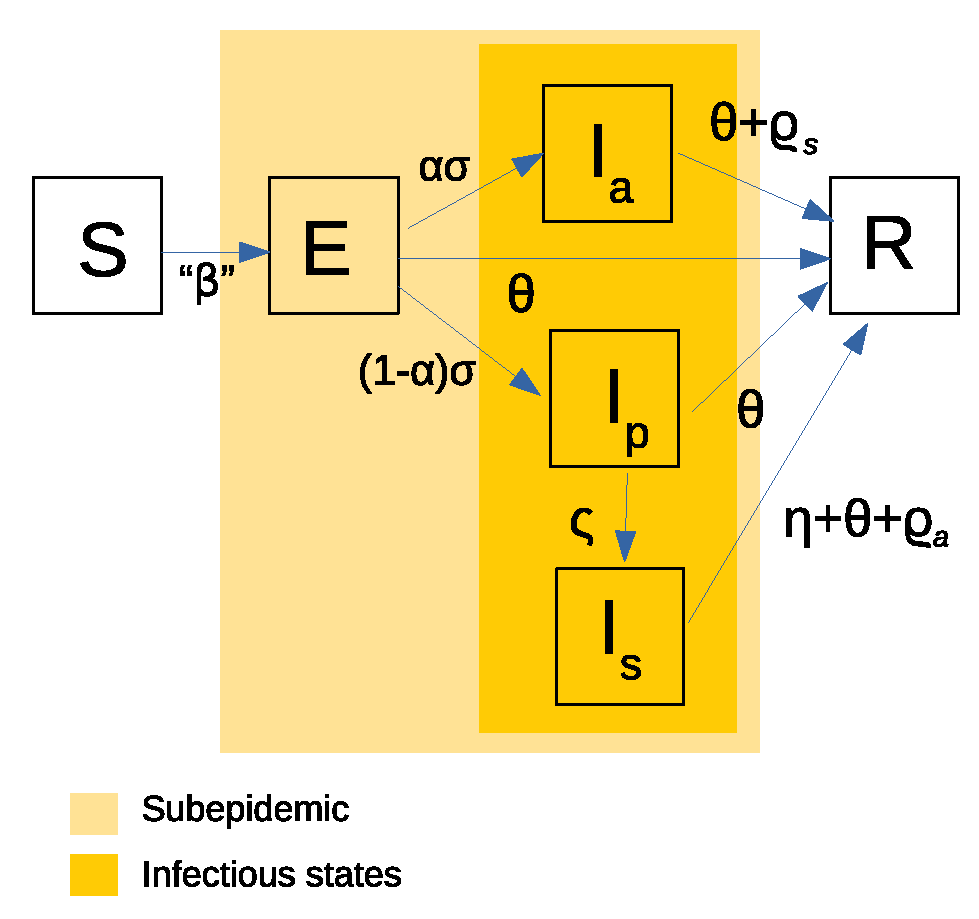
\includegraphics[scale=0.3,bb = 0 0 200 100, draft, type=eps]{simple.eps}
\par\end{center}

If we neglect (small) joint probabilities of natural exits from the
infectious states and the isolations, we get 
\[
P_{t}=\left[\begin{array}{ccccc}
1-\sigma-\theta_{t}^{e} & 0 & 0 & 0 & 0\\
\alpha\sigma & 1-\varrho_{a}-\theta_{t}^{a} & 0 & 0 & 0\\
(1-\alpha)\sigma & 0 & 1-\varsigma-\theta_{t}^{p} & 0 & 0\\
0 & 0 & \varsigma & 1-\varrho_{s}-\eta-\theta_{t}^{s} & 0\\
\theta_{t}^{e} & \theta_{t}^{a}+\varrho_{a} & \theta_{t}^{p} & \theta_{t}^{s}+\eta+\varrho_{s} & 1
\end{array}\right],\qquad B_{t}=\left[\begin{array}{ccccc}
0 & \beta_{t} & \beta_{t} & \beta_{t} & 0\\
0 & 0 & 0 & 0 & 0\\
0 & 0 & 0 & 0 & 0\\
0 & 0 & 0 & 0 & 0\\
0 & 0 & 0 & 0 & 0
\end{array}\right]
\]
Clearly, we can put $m=4$ (the first four states form a sub-epidemic),
getting 
\[
\barT_{t}=Q+\beta_{t}C-\mathrm{diag}(\theta_{t}),\qquad Q=\left[\begin{array}{cccc}
1-\sigma & 0 & 0 & 0\\
\alpha\sigma & 1-\varrho_{a} & 0 & 0\\
(1-\alpha)\sigma & 0 & 1-\varsigma & 0\\
0 & 0 & \varsigma & 1-\varrho_{s}-\eta
\end{array}\right],\qquad C=\left[\begin{array}{cccc}
0 & 1 & 1 & 1\\
0 & 0 & 0 & 0\\
0 & 0 & 0 & 0\\
0 & 0 & 0 & 0
\end{array}\right]..
\]
Further we assume $\theta_{t}\defined\theta_{t}^{e}=\theta_{t}^{a}=\theta_{t}^{p}=\theta_{t}^{s}$,
which yields, by the well known rule, $\rho(\barT_{t})=\rho(Q+\beta_{t}C)-\theta_{t}$.
We consider two ways of decreasing the spectral radius: decreasing
the infection rate $\beta_{t}$ (typically by wide counter-epidemic
measures) and increasing the isolation rate $\theta_{t}$ (e.g. by
strengthening the testing and tracing capacity).

Once there is a ``target'' spectral radius $\rho_{0},$ all the
combinations of $\beta$ and $\theta$ yielding $\rho(\barT_{t})=\rho_{0}$
fulfill $\rho_{0}+\theta-\rho(Q+\beta_{t}C)=0,$which gives a ``marginal
rate of substitiution'' $\theta(\beta)'=-\frac{\partial}{\partial\beta}\rho(Q+\beta_{t}C)$
of the infectiousness by the isolation, i.e. how much we have to increase
the isolation speed when we release the restrictions.
\end{example}

\begin{example}
Assume there is a fraction $\nu$ of the population is non-compliant,
which means that, once a restriction on social contacts is imposed,
they apply it only partially. Assume that, without restrictions, the
population is mixed which means that each individual, compliant or
not, has, up to a constant, $(1-\nu)$ contacts with the compliant
individuals and $\nu$ contacts with the non-compliant ones. Once
there is a measure imposed under which the compliant individuals restrict
their opportunities to contacts by $\phi$, the non-compliant ones
do so only to $f(\phi)>\phi$ . As a result, the compliant ones will
have, up to a constant, $\phi^{2}(1-\nu)$ contacts with the compliant
ones, $\phi f(\phi)\nu$ contacts with the non-compliant ones, while
the non-compliant will have $\phi f(\phi)(1-\nu)$ and $f(\phi)^{2}\nu$
contacts with the compliant, non-compliant, respectively.

Assuming a simple epidemic model with compartments $I_{c}$ - infected
compliant, $I_{n}$ - infected non-compliant, and $R$ - removed,
with the course of infection being the same for both the compartments
such that $\beta_{t}^{1i}=\beta c_{i}$, $i\in\{1,2\},$ where $\beta$
is a constant and $c_{i}$ is the number of contacts of the $i$-th
sub-population, this gives 
\[
P_{t}=\left[\begin{array}{ccc}
1-\varrho & 0 & 0\\
0 & 1-\varrho & 0\\
\varrho & \varrho & 1
\end{array}\right],\qquad B_{t}=\left[\begin{array}{ccc}
\beta\phi^{2}(1-\nu) & \,\beta\phi f(\phi)\nu\, & 0\\
\beta\phi f(\phi)(1-\nu) & \,\beta f(\phi)^{2}\nu\, & 0\\
0 & 0 & 1
\end{array}\right]
\]
where $\varrho$ is a removal rate (perhaps consisting of an artificial
and a natural part). This gives 
\[
\barT_{t}=\beta C+(1-\varrho)E,\qquad C=\left[\begin{array}{cc}
\phi^{2}(1-\nu) & \,\phi f(\phi)\nu\\
\phi f(\phi)(1-\nu) & \,f(\phi)^{2}\nu
\end{array}\right]
\]
with 
\[
\varrho(\barT_{t})=\beta\rho(C)+(1-\varrho).
\]
As the characteristic polynomial of $C$ is 
\[
\lambda^{2}-\lambda g,\qquad g=g(\phi,\nu)=\phi^{2}(1-\nu)+f(\phi)^{2}\nu
\]
we clearly have $\rho(C)=g.$

Now say that our goal is to decrease $\rho(\barT_{t})$ to a predetermined
value $r$ by finding appropriate $\phi=\phi(\nu)$. In order to do
so, we have to solve
\[
\beta g(\phi(\nu),\nu)+(1-\varrho)=r.
\]
Clearly, $\phi(0)=\phi_{0}\defined\sqrt{\frac{r-1+\varrho}{\beta}}$.
For $\nu>0$ we get, by the Implicit function theorem, 
\[
\frac{\partial}{\partial\nu}\phi=\frac{f(\phi(\nu))^{2}-\phi(\nu)^{2}}{2\phi(\nu)(1-\nu)+2f(\phi(\nu))f'(\phi(\nu))\nu}.
\]
Note that the derivative depends neither on $r$ nor on $\varrho$
. Thus we can easily compute how the non-compliance influences strictness
of the necessary restrictions. For instance, by the first-order Taylor
expansion at $\nu=0$, we get 
\[
\phi(\nu)\doteq\phi_{0}+\nu\frac{f(\phi_{0})^{2}-\phi_{0}^{2}}{2\phi_{0}}=\phi_{0}\left(1-\frac{\nu}{2}\right)+\nu\frac{f(\phi_{0})^{2}}{2\phi_{0}}
\]
roughly holding for $\nu$ close to zero.
\end{example}


\section{Cohort Model\label{sec:cohorts}}

In the present Section, we assume the population to be split into
$r$ (age) cohorts of sizes $s_{1},\dots,s_{r}$, $s_{1}+\dots+s_{r}=s$.
The members of each cohort may be either susceptible or belong to
one of $\kappa$ analogous compartments. Naturally assuming that individuals
do not migrate between cohorts, we get the overall transition matrix
as 
\[
P_{t}=\left[\begin{array}{cccc}
P_{t}^{1} & 0 & \cdots & 0\\
0 & P_{t}^{2} & \cdots & 0\\
\vdots & \vdots & \ddots & 0\\
0 & 0 & \cdots & P_{t}^{r}
\end{array}\right]
\]
where $P_{t}^{i}$ are $\kappa\times\kappa$ cohort transition matrices,
$1\leq i\leq\kappa$, $t\geq0$. Note that once there are dispersion
parameters $c_{1}^{i},\dots,c_{\kappa}^{i}$ associated with each
matrix $P_{t}^{i}$ (meaning that, once the $j$-th compartment of
the $i$-th cohort is of size $x$, the transfers from the cohort
to the cohort's compartments follow $\mathrm{DM}(x,\frac{(P^{i})^{(j)}}{c_{i}^{j}})$),
the dispersion parameters of the overall model are $(c_{1}^{1},\dots,c_{\kappa}^{1},c_{1}^{2},\dots c_{\kappa}^{2},c_{1}^{3},\dots\dots,c_{\kappa}^{r}).$

We assume that the contagions can happen across cohorts. Namely, the
probability of contagion, i.e. the transfer of a susceptible individual
to the $i$-th compartment of the $p$-th cohort, upon a risk contact
with a member of the $j$-th compartment of the $q$-th cohort does
not depend on $p$ or $q$, being equal to $\varpi_{t}^{ij}$. Further
we assume that, on average, a member of the $p$-th cohort has $\nu^{pq}$
risk contacts with the $q$-th cohort, assuming that the number of
contacts with the infectious compartments (those with non-zero $\varpi_{t}^{i\bullet})$
is equal. Under these assumption, the probability a transfer of a
susceptible individual from cohort $p$ into the $i$-th compartment
is roughly $e_{t}^{pi}\defined b\sum_{q=1}^{r}\sum_{j=1}^{k}\nu^{pq}\varpi_{t}^{ij}\frac{X_{tq}^{i}}{s_{q}}$,
where $X_{tq}^{i}$ is the size of the $i$-th compartment of cohort
$q$ and $b$ is a constant. Consequently, the total number the infections
in the $i$-th compartment of the $p$-th cohort will be $s_{p}e_{t}^{pi}$,
which gives 
\[
B_{t}=Q\otimes C_{t}
\]
where 
\[
Q=\left[\begin{array}{cccc}
\nu^{11} & \nu^{12}\frac{s_{1}}{s_{2}} & \cdots & \nu^{1r}\frac{s_{1}}{s_{r}}\\
\nu^{21}\frac{s_{2}}{s_{1}} & \nu^{22} & \cdots & \nu^{2r}\frac{s_{2}}{s_{r}}\\
\vdots & \vdots & \ddots & \vdots\\
\nu^{r1}\frac{s_{r}}{s_{1}} & \nu^{r2}\frac{s_{r}}{s_{2}} & \cdots & \nu^{rr}
\end{array}\right],\qquad C_{t}=\left[\begin{array}{cccc}
\varpi_{t}^{11} & \varpi_{t}^{12} & \cdots & \varpi_{t}^{1k}\\
\varpi_{t}^{21} & \varpi_{t}^{22} & \cdots & \varpi_{t}^{2k}\\
\vdots & \vdots & \ddots & \vdots\\
\varpi_{t}^{k1} & \varpi_{t}^{k2} & \cdots & \varpi_{t}^{kk}
\end{array}\right].
\]


\section{Optimal Control of the Epidemics\label{sec:oc}}

Assume the setting of Example \ref{exa:e1} and assume that $X_{0}$
is known. Our aim is to minimize the size of the epidemic at time
$t$ given that we are ready to pay a given price $c_{0}$. We assume
that, to achieve infection rate $\beta$, a cost $\gamma(\beta)$
has to be paid where $\gamma$ is a strictly decreasing convex positive
function defined on $(0,\beta_{0}]$ with $\gamma(\beta_{0})=0$ and
$\gamma(0-)=\infty$. Further, to achieve the isolation rate $\theta_{t}^{i}$
in the $i$-th compartment, the price $\delta(\theta_{t}^{i},X_{t}^{i})\defined d\theta_{t}^{i}X_{t}^{i}$
has to be paid where $d$ is a constant. This reflects the real-life
situation in which the cost of global restrictions does not depend
on the infection size while the cost of isolation does, for instance
through the number of call-center workers involved in tracing. 

Our problem is to find 

\[
V_{0}(X_{0},c_{0})\defined\inf_{\sum_{\tau=0}^{t-1}[\gamma(\beta_{\tau})+\delta(\theta_{t}^{k},X_{t}^{k})+\dots+\delta(\theta_{t}^{k},X_{t}^{k})]\leq c_{0},\beta,0\leq\theta\leq q,\theta_{\tau}\in\F_{\tau},\beta_{\tau}\in\F_{\tau},1\leq\tau<t}\E(\mathbf{1}'X_{t})
\]
where $q$ is the diagonal of $Q.$ The problem may be rewritten by
means of Bellman equations 
\begin{align*}
V_{\tau}(x,c) & =\inf_{\gamma(\beta)+d\theta^{k}x^{k}+\dots+d\theta^{k}x^{k}+y\leq c,\beta\geq0,\theta\geq0,y\geq0}\E(V_{\tau+1}(J,y)),\qquad0\leq\tau<t,
\end{align*}
\[
V_{t}(x,c)=\mathbf{1}'x,
\]
\[
J\sim\L(x,\beta,\theta)\defined\bigcirc_{1\leq i\leq m}\mathrm{Multinomial^{-}}(x^{i},Q^{(i)}-\Delta_{i}\theta^{i})\circ\mathrm{Po}(\beta Cx)
\]
where $\Delta_{i}$ is the vector with the unit component on the $i$-th
place and zeros otherwise.

Though the final problem is convex --
\begin{multline*}
V_{t-1}(x,c)=\inf_{\gamma(\beta)+d\theta^{1}x^{1}+\dots+d\theta^{m}x^{m}+y\leq c,0\leq\theta\leq q,\beta,y\geq0}\mathbf{1}'(Qx-\mathrm{diag}(\theta)x+\Delta_{e}\beta\sum_{i\neq e}x^{i})
\end{multline*}
-- its objective function is not jointly convex in $(u,v,x,c)$,
so the convexity of $V_{t-1}$ is not guaranteed. Moreover, as neither
the optimal solution nor the expectation of the objective functions
of all but the last problem are analytically tractable, it is necessary
to resort to approximations. To this end, we can use the sample mean
approximation 
\[
V_{\tau}(x,c)\doteq\tilde{V_{\tau}}(x,c)
\]
 where $\tilde{V}_{t}=V_{t}$ and, recursively,
\[
V_{\tau}(x,c)\doteq\tilde{V_{\tau}}(x,c)\defined\inf_{\gamma(\beta)+d\theta^{k}x^{k}+\dots+d\theta^{k}x^{k}+y\leq c,\beta,\theta,y\geq0}\frac{1}{r}\sum_{i=1}^{r}\tilde{V}_{\tau+1}(J_{i},y)
\]
where $J_{1},\dots,J_{r}$ is an i.i.d. sample from $\L(x,\beta,\theta)$.

\section{Estimation}

\label{sec:Estimation}For any stochastic process $A$ and integers
$s\geq t$, denote $\hat{A}_{s|t}=\E(A_{s}|\G_{t})$. Let $s>t$.
When $T_{\tau}\in\G_{t},t<\tau\leq s-1$ (which is trivially true
if $s=t+1$), we get that

\begin{multline*}
\left[{\hat{X}_{s|t}\atop \hat{Y}_{s|t}}\right]=\E\left(\left.\E\left(\left.\left[{X_{s}\atop Y_{s}}\right]\right|\F_{s-1}\right)\right|\G_{t}\right)=\left[{E\atop F}\right]\left(T_{s-1}\hat{X}_{s-1|t}+\hat{I}_{s-1|t}\right)\\
=\left[{E\atop F}\right]\left(T_{t,s-1}X_{t}+\sum_{\theta=t}^{s-1}T_{\theta+1,s-1}\hat{I}_{\theta|t}\right),
\end{multline*}
\begin{multline*}
W_{s|t}\defined\var\left(\left.X_{s}\right|\G_{t}\right)=\var\left(\left.\E\left(\left.X_{s}\right|\F_{s-1}\right)\right|\G_{t}\right)+\E\left(\left.\var\left(\left.X_{s}\right|\F_{s-1}\right)\right|\G_{t}\right)\\
=\var\left(T_{s-1}X_{s-1}+I_{s-1}|\G_{t}\right)+\E\left(\left.\Lambda_{s-1}(X_{s-1},X_{s-1}^{2})\right|\G_{t}\right)\\
=T_{s-1}W_{s-1|t}T_{s-1}^{T}+2T_{s-1}\cov(X_{s-1},I_{s-1}|\G_{t})+\var\left(I_{s-1}|\G_{t}\right)\\
+\Lambda_{s-1}(\hat{X}_{s-1|t},\mathrm{diag}(W_{s-1|t})+\hat{X}_{s-1|t}^{2})
\end{multline*}
(we have used linearity of $\Lambda_{s-1}$, thanks to which $\E(\Lambda_{s-1}(\hat{X}_{s-1|t},X_{s-1}^{2})|\G_{t})=\Lambda_{s-1}(\E(X_{s-1}|\G_{t}),\E(X_{s-1}^{2}|\G_{t}$)),
and the well known formula $\var(X)=\E X^{2}-(\E X)^{2})$. Consequently,
\begin{multline*}
V_{s|t}\defined\var\left(\left.{X_{s}\atop Y_{s}}\right|\G_{t}\right)=\var\left(\left.{X_{s}\atop FX_{s}+\epsilon_{s}}\right|\G_{t}\right)\\
=\left[{E\atop F}\right]W_{s|t}\left[{E\atop F}\right]^{T}+\mathrm{diag}\left({0_{k}\atop \Gamma_{s-1}(\hat{X}_{s-1|t},\mathrm{diag}(W_{s-1|t})+\hat{X}_{s-1|t}^{2})}\right)
\end{multline*}
Unfortunately, due to the non-Gaussianity, we have analytical formulas
for none of $X_{t|t}$ $I_{t|t}$ and $\mathrm{W_{t|t}}$, so we can
formulate neither the likelihood function nor a least square estimate.
Two, from the computational point of view equivalent, ways to cope
with this are using estimates of the conditional expectation and variance,
or normally approximating the residuals. We go the latter way: in
the present Section, we assume that $\left.\left[{X_{t+1}\atop Y_{t+1}}\right]\right|\F_{t}$
is normal with mean given by (\ref{eq:mean}) and 
\[
\var\left(\left.{X_{t+1}\atop Y_{t+1}}\right|\F_{t}\right)=\left[{E\atop F}\right]\Lambda_{t}(X_{t}\vee0,X_{t}^{2})\left[{E\atop F}\right]^{T}+\mathrm{diag\left({0_{k}\atop \Gamma_{t}(X_{t}\vee0,X_{t}^{2})}\right)}
\]
Moreover, we assume that $I_{t}\in\G_{t},t\geq0$ (i.e. the import
is observable). Given these assumptions, we have, by the well known
formula (see e.g. \cite{Eaton07}), 
\begin{multline*}
\hat{X}_{t|t}=I_{t-1}+\hat{X}_{t|t-1}+K_{t}\left(Y_{t}-\hat{Y}_{t|t-1}\right),\qquad K_{t}\defined\tilde{V}_{t|t-1}^{XY}(\tilde{V}_{t|-1}^{YY})^{-1}
\end{multline*}

\begin{multline*}
\var(X_{t}|\G_{t})=\tilde{V}_{t|t-1}^{XX}-\tilde{V}_{t|t-1}^{XY}(\tilde{V}_{t|t-1}^{YY})^{-1}\tilde{V}_{t|t-1}^{YX}
\end{multline*}
where $\tilde{V}_{s|t}\defined\var(\left[{X_{s}\atop Y_{s}}\right]|\G_{t})$
given the normal approximation. Note that $K_{t}$ may be seen as
a conditional version of the Kalman gain matrix. 

If $\P[\hat{X}_{t}<0]$ is negligible (which is typically true when
modeling large epidemics), then we can neglect truncation in the formula
for the variance approximate $\tilde{V}_{t|s}\doteq V_{t|s},$which
further gives 

\begin{multline*}
K_{t}\doteq W_{t|t-1}F^{T}D_{t}^{-1},\qquad D_{t}=FW_{t|t-1}F^{T}+\mathrm{diag}(\Gamma_{t}\hat{X}_{t|t-1})
\end{multline*}

\begin{multline*}
W_{t|t}\doteq W_{t|t-1}-W_{t|t-1}F^{T}D_{t}^{-1}FW_{t|t-1}
\end{multline*}

Assume that $F=F(\Theta_{0}),$$P_{t}=P_{t}(\Theta_{0})$, $B_{t}=B_{t}(\Theta_{0})$,
$\Gamma_{t}=\Gamma_{t}(\Theta_{0})$ and $I_{t}=I_{t}(\Theta_{0})$,
and $c=c(\Theta_{0})$, where $\Theta_{0}\in\R^{r}$ is an unknown
parameter. For its estimation, it is possible to use either nonlinear
least squares, i.e. 
\[
\hat{\Theta}=\arg\min\sum_{t}(Y_{t}-\hat{Y}_{t|t}(\Theta))^{T}U_{t}(Y_{t}-\hat{Y}_{t|t}(\Theta))
\]
where $U_{t}\in\G_{t-1}$ is a suitable weighting matrix, or 
\[
\tilde{\Theta}=\arg\min\sum_{t}\varphi(Y_{t}-\hat{Y}_{t|t}(\Theta),D_{t}(\Theta)),\qquad\varphi(x,v)=-\frac{k\ln2\pi+\ln\mathrm{det}(v)+x^{T}v^{-1}x}{2}
\]
Both these estimators are consistent and asymptotically normal under
some conditions, see \cite{Jacob10}, \cite{jacob2013generalized},
respectively. Verifying these conditions for our model is, however,
beyond the scope of this introductory study and remains as topic of
a future research. 

It should be noted that our proof of Proposition \ref{prop:as} is
not valid for the approximate model, as $\barX$ is not necessarily
positive given the Normal approximation.

\section{Application to The COVID Pandemics in the Czech Republic}

\label{sec:Application-to-The}We applied our model to the data from
the pandemics in the Czech Republic between February 2020 and January
2021. We considered a widely generalized version of the model from
Example \ref{exa:e1}, compartments of which are shown in Figure \ref{fig:big}:
\begin{center}
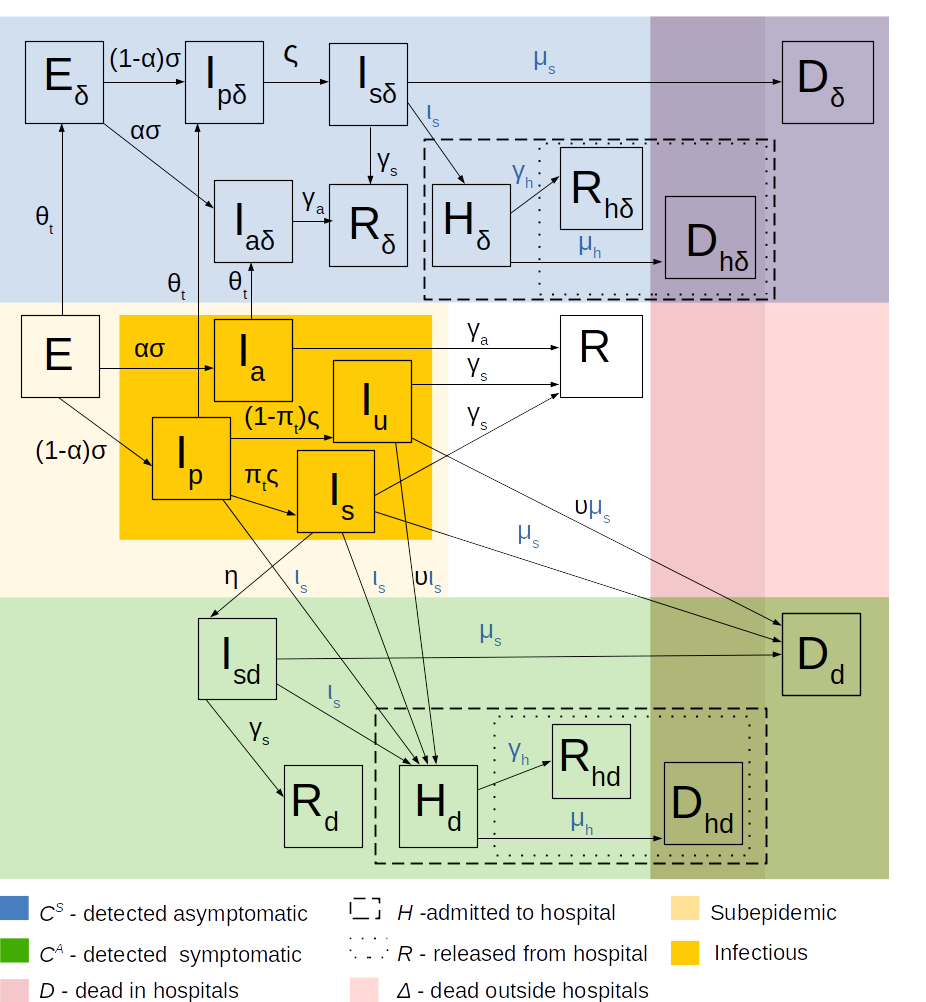
\includegraphics[scale=0.3]{big}
\par\end{center}

\label{fig:big}

To reflect the fact that many cases are (intentionally) undetected,
we added the compartment $I_{u},$ members of which can be detected
only if they get to hospital or die, otherwise they never undergo
testing. Further, to all the compartments from Example \ref{exa:e1}
we added their ``detected'' versions, distinguishing detection when
being asymptomatic (subscript $\delta$) or symptomatic (subscript
$d$). We distinguish three ``removed'' states: recovered ($R$),
hospitalized ($H$) and dead ($D$). Assuming that each individual
who gets to the hospital is detected upon entry, we have two versions
of $H$ states: detected when symptomatic ($H_{d}$) and detected
when asymptomatic ($H_{\delta})$. Similarly we assume that each dead
is detected and we distinguish whether the individual dies in- or
outside of hospital; consequently, we have four ``dead'' states:
$D_{hd},D_{d},$$D_{h\delta}$ and $D_{\delta}.$ The case of $R$
is analogous with the exception that recovery can happen without detection,
so we have five versions: $R,$$R_{dh}$, $R_{d},$$R_{\delta h}$,
and $R_{\delta}.$ 

We distinguish four age cohorts: $0$ to $19$ years, $20$ to 64
years, $65$ to $79$ years and more than $80$ years; consequently,
having four compartments for each state, we have $4\times21=84$ compartments
in total. 

Some transition parameters (components of $P_{t})$ are common for
the compartments (black symbols in Figure \ref{fig:big}) and partially
specific for each compartment (blue symbols). Some parameters are
constant in time, some (those with index $t$) are time varying. The
values of some parameters were externally determined, some were estimated.
The detailed description of parameters, way of their determination,
computation or estimation, and their estimated values may be found
in Appendix. Here we only mention that we take
\[
\theta_{t}=\vartheta_{0}+\vartheta_{1}q_{t},
\]
where $q_{t}$ is the observed probability, that an infectious individual
is accepted to hospital without being previously detected, which,
as of February 2021, serves as an input of the national counter-epidemic
system, and, by the Bayes rule, it is, up to a constant, equal to
the overall detection probability. The rate $\pi_{t}$ is set so as
the the detection probability holds in the model (see the Appendix). 

The normalized ``mixing matrix'' $Q$ has been computed from the
estimate of the overall contact matrix in the Czech by \cite{prem2017projecting},
see the Appendix. 

In line with \cite{pollock2020asymptomatic}, reporting $3-25$ tines
lower secondary attack rate of asymptomatic individuals, we assume
that the probability of infection by $I_{a}$ is four-times less in
comparison with $I_{p},$$I_{s}$ and $I_{u},$ we assume the dependence
of infectiousness on the contact restriction and personal protection,
and we reflect the natural immunization. Namely, we put
\[
\varpi_{t}^{EI_{s}}=\varpi_{t}^{EI_{\acute{u}}}=\varpi_{t}^{EI_{s}}=\varpi_{t},\qquad\varpi_{t}^{EI_{a}}=\frac{1}{4}\varpi_{t},\qquad\varpi_{t}^{\bullet}=0\text{ otherwise,}
\]
\begin{equation}
\varpi_{t}=g_{t}h_{t}\upsilon_{t-7}p_{t-7}\label{eq:gamma}
\end{equation}
where $\upsilon_{t}$ is the average number of risk contacts and $p_{t}$
is the reduction caused by personal protection, $h_{t}\defined1-\frac{\sum_{i=1}^{k}\hat{X}_{t|t}^{i}}{s}$
is the adjustment for immunization (we assume that once infected cannot
be infected again) and $g_{t}$ is the adjustment for new mutation,
see Appendix for details. 

The values $\upsilon_{t}$ and $p_{t}$, were taken from \cite{paqcovid}
which is a longitudinal study, inquiring a panel of 3000 respondents
about their (weekly) risk contacts, observance of several personal
protection measures (see Appendix), and some other variables. While
the value $\upsilon_{t}$ is being directly questioned by the survey,
we compute the level $p_{t}$ of personal protection as $p_{t}=\omega_{0}\exp\{-\omega_{e}e_{t-7}-\omega_{f}f_{t-7}\}$
where $e_{t}$ is a certain linear combination of observation rates
of various personal protective measures, $f_{t}$ is the reported
level of fear caused by the pandemic and $\omega_{0},\omega_{e}$
and $\omega_{f}$ are constants - see Appendix for further explanation.

For better comparison with other models, we use normalized version
of the personal contacts level $w_{t}\defined\frac{\upsilon_{t}}{\upsilon_{0}}$
where $\upsilon_{0}$ is the pre-pandemic value of $\upsilon,$ so
we have
\[
\varpi_{t}=g_{t}h_{t}w_{t-7}\exp\{-\omega_{e}e_{t-7}-\omega_{f}f_{t-7}\}
\]
up to constant multiplication, where the corresponding constant becomes
part of estimated parameters $b_{0},b_{20},b_{65}$ and $b_{80}$ 

As for the dispersion parameters, we assume $v=26$ (see Remark \ref{rem:-v})
and, for each cohort $i,$ $c_{x}^{i}\equiv c_{h}$, $x\in\{H_{d}^{i},H_{\delta}^{i}\}$
(all ``hospital'' states) and $c_{x}^{i}\equiv c_{a}$ otherwise
-- both $c_{h}$ and $c_{a}$ are estimated. This restriction of
the parameter space was chosen in order to avoid overparametrization,
but to reflect the larger variability of incidences and hospitalizations
in comparison with the mortality data (note that dead mostly come
from hospitals). Note also that for terminal states the dispersion
parameters have no effect, as their ``target'' distribution is Dirac.

We use the following daily data series: 
\begin{description}
\item [{$\tilde{I}^{0},\tilde{I}^{20},\tilde{I}^{65},\tilde{I}^{80}$}] -
imports to individual cohorts,
\end{description}
and, as observations (variables $Y$): 
\begin{description}
\item [{$C^{A},C^{S}$}] - incidences of asymptomatic, symptomatic, respectively
\item [{$C^{0},C^{20},C^{65},C^{80}$}] - incidences in individual cohorts
\item [{$D^{0},D^{20},D^{65},D^{80}$}] - deaths in individual cohorts
\item [{$H^{y},H^{o}$}] - admissions to hospitals of individuals from
the first two cohorts, second two cohorts, respectively
\item [{$R^{y},R^{o}$}] - number of released from hospitals of the first/second
two cohorts
\item [{$D^{y},D^{o}$}] - dead in hospitals of the first/second two cohorts
\item [{$\Delta^{y},\Delta^{o}$}] - dead outside hospitals of the first/second
two cohorts
\end{description}
The data come from the public repository of the Ministry of Health
of the Czech Republic and from the The Institute of Health Information
and Statistics of the Czech Republic, where the former is publicly
available while the latter is available only to research institutions.
See Figure {[}fig:inputs{]} for overview. 

The data had to be per-processed. First of all, series $C$, $H$
and $R$, showing strong weekly pattern, have been de-seasoned. Second,
as the total reported incidence exceeds by $2$ percent the personal
level data (probably because details are not always known), we took
the former as decisive. Next, as the reports of symptomatic an asymptomatic
results of tests give slightly less total then the incidence, we took
only ratios from the former multiplied by titak incidences as $C^{a}$
and $C^{s}$ Finally, as the total reported number of actually hospitalized,
which we denote by $L$, exceeds (by units of per-cents) the totals
from the anonymized hospitalization data, we adjusted series $H$
and $R$ so that $L\doteq H-R$ (doing it exactly is impossible, as
plain multiplication could cause unrealistic values of $H$ and $R$).

The matrix $F$ transferring compartment sizes $X$ to observables
$Y$, is zero-one. Which components are one can be paritally devised
from Figure \ref{fig:big}, its exact definition finds itself in Appendix.
The lack of a row of $F$ corresponding to $C^{A}$ is intentional
as $C^{A}$ is redundant (equal to $C^{0}+C^{20}+C^{65}+C^{80}-C^{S}$)
and would cause linear dependence in $F$.

Assuming the imports only to the state $E$, we take, 
\[
I_{t}^{i}=\tilde{I}_{t+8}^{i}
\]
for each cohort $i$ (the time-shift reflects the delay in reporting).

Reflecting the notorious unreliability of incidence data, we put 
\[
\Gamma_{t}(x,y)=\mathrm{diag}(\gamma_{s},\gamma_{c},\gamma_{c},\gamma_{c},\gamma_{c},0,\dots,0)Fx
\]
where $\gamma_{s}$ and $\gamma_{c}$ are estimated parameters (note
that the first five rows of $F$ correspond to $C^{S},C^{0},C^{20},C^{65},C^{80}$
respectively.

For estimation, we used Weighted least squares applied to the seven
day forecasts with weekly average increments as weights: 
\[
U_{t}=\mathrm{diag}\left(\left(\frac{Y_{t}^{i}-Y_{(t-7)\vee0}^{i}}{7\wedge t}\vee5\right)_{i=1}^{n}\right),\qquad t>0.
\]
Due to the possibly different nature of the first wave (until May)
and irregular behavior of the pandemic in summer (caused by small
incidence with local outbursts), we used only data from October onward
for the (final) estimation. To get ``reasonable'' initial state
for our estimate, we roughly estimated the model for the whole period
of the pandemic and took its state from the end of August as the initial
state for the final estimation; the WLS estimate, however, was computed
only from period October 1, 2020 till January 21, 2121 (to minimize
the influence of the initial value). 

Unfortunately, the estimation did not directly lead to quality results.
The reason was that running the minimization with free $c_{u},c_{d},\gamma_{s}$
and $\gamma_{c}$ (dispersion) parameters tends to underestimate forecast
variances, which fact subsequently leads to unrealistically narrow
confidence bounds. In order to get more realistic variances, we, by
a grid search, adjusted the risk parameters so that the variance of
standardized (one day forecast) residuals were close to one, then
re-estimated the model by WLS with the adjusted risk parameters fixed.
Yet the value of the new WLS minimum is about 6 percent higher than
the original one, the variances in the new model are realistic. Finding
a fully automatic estimation procedure getting realistic variances,
perhaps by regularization with respect to variance of residuals, is
a challenging topic of future research. The C++ code for the WLS estimation,
emplying NLopt library for minimization, is available on https://github.com/cyberklezmer/seir/tree/ejor. 

The standardized residuals of seven-day predictions (i.e. the residuals
divided by the standard error of the estimate) for the individual
observables, may be seen in Figure fig:residuals. Figure fig:forecasts,on
the other hand, shows the predictions fit of the total incidence $C_{t}\defined C_{t}^{0}+C_{t}^{20}+C_{t}^{65}+C_{t}^{80},$
the total number of deaths $D_{t}\defined D_{t}^{0}+D_{t}^{20}+D_{t}^{65}+D_{t}^{80}$
and the actual occupancy of hospitals $L_{t}\defined H_{t}^{y}+H_{t}^{o}-R_{t}^{y}-R_{t}^{o}.$
For each variable, the left-hand graph shows the fit of the (in-sample)
seven day predictions, the right-hand graph the (out of sample) predictions
for 14 days following Jan 21. 

\section{Vaccination Experiment}

\label{sec:Vaccination-Experiment}Finally, as a demonstration of
applicability of our model, we evaluated outcomes of three vaccination
scenarios
\begin{description}
\item [{novac}] The infectiousness $\varpi_{t}$ increases by 50\% on January
22 (by emergence of a new mutation and/or release of the counter-epidemic
measures) and keeps being constant until the end of May 
\item [{elderly}] The infectiousness rises as above, but 30000 shots of
vaccine a day will start to be applied on February 1st. Vaccines are
distributed to the cohort 80+ first and, as late as all the cohort
is vaccinated, vaccines start to be given to cohort 65-79. After 35
days, each vaccinated individual gets a second shot (these shots do
not count to the daily number 30000). 
\item [{middle}] The situation is the same as in ``elderly'' scenario
with the difference that only 15000 vaccines a day are given to the
oldest, the rest are gien to cohort 20-64 (perhaps infrastructural
workers).
\end{description}
As for the vaccine effect, we (conservatively) assume that vaccinated
individuals can be infected the same way as if they were not vaccinated;
however, the probability of the asymptomatic course rises: 14 days
after the first shot to $0.9$ for the first two cohorts (0-64), or
to 0.7 for those who are older than 65. After 14 days from the second
shot, the probability further rises to 0.8, 0.95, respectively.

The results of simulation are shown in Figure TBD and Table TBD. Not
surprisingly, vaccination saves all the infections, deaths and hospital
beds. Prioritizing the older saves lives and beds, however, adds infections
(which partially due to greater efficiency of the vaccine for the
younger cohorts, maybe also due to greater number of contacts of the
young). The most important message, however, is that vaccination is
not a ``silver bullet'' solving everything -- there still large
number of dead with vaccination, which could be saved if the infectiousness
was reduced, too, perhaps by some unpopular measures.

.

\section{Conclusion}

\label{sec:Conclusion} We presented a stochastic epidemic model,
formulated its basic properties and suggested way of its estimation,
all demonstrated by a real-life examples. We demonstrated that our
model has good prediction power. They are, however, many things to
be done. Most importantly, a reliable automatic estimation procedure
should be suggested, guaranteeing good fit of both means and variances.
Second, regularity conditions which would assure asymptotic properties
should be formulated, yet it can be a difficult task.. However, even
as it is, it can be immediately used for statistically correct modeling
of the epidemics. 

\bibliographystyle{plain}
\bibliography{/home/martin/Documents/s/smid,covid_m}


\section*{Parameters of the Czech Republic Model}

The following Table lists the values, serving for computation of the
former.

\begin{center}
\begin{tabular}{lll} \hline Par.&	description&	Source \\ \hline\hline 
$m_E=5.08$ & mean of incubation period &		\cite{he2020estimation}	
\\
$\alpha = 0.179$ & probability of asymptomatic course & \cite{mizumoto2020estimating}
\\
$m_a=4$ & expected duration of presymptomatic period
&	\cite{nie2020epidemiological} 
\\
 $m_i = 8$ & expected duration of infectiousness 
	&	\cite{Wolfel2020virological}	\\ 
%\\ 
% r=0.018 & case fatality ratio & \cite{he2020estimation}
	\\ \hline \end{tabular} \end{center}

Assuming the compartment occupation times to be exponential, we get
the following transition probabilities:

\begin{center}
\begin{tabular}{l} \hline Par. \\ \hline\hline 
$\sigma=1-\exp\{-1/m_E\}$ 
\\
$\varsigma = 1-\exp\{-\frac{1}{m_a}\}$ 
\\
$\gamma_s=1-\exp\{-\frac{1}{m_s}\}$ 	\\ 
$\gamma_a = 1-\exp\{-\frac{1}{m_i+m_a}\}$ \\
$\mu$ - estimated \\
%\\
% $\mu=r(1-\exp\{\frac{1}{m_s-m_i-m_a}\})$
	\\ \hline \end{tabular} 
\end{center}

y

y

y

The parameters, not included in Table \ref{tab:params}
are $\theta_{t}$, which is defined by \ref{eq:theta},
$\pi_{t}$, which we define later, and $\varpi_{t}$ which is defined
by (\ref{eq:varpi}) but with owing explanation how
$p_{t}$ is computed.

The quantity $\pi_{t}$ is set so that the overall detection probability,
which we estimate by $\delta q_{t}$ where $q_{t}$ is discussed in
the main text and $\delta$ is an estimated parameter. If we assume
that, through time, the states of an individual follows a \emph{continuous-time}
Markov chain with transition matrix given by parameters, listed in
Figure \ref{fig:big}, then the probability of detection
(excluding the cases when an undetected arrives to hospital or dies)
is
\begin{multline*}
d_{t}\defined\P[E\rightarrow E_{\delta}\vee E\rightarrow I_{a}\rightarrow I_{a\delta}\vee E\rightarrow I_{p}\rightarrow I_{p\delta}\vee E\rightarrow I_{p}\rightarrow I_{s}\rightarrow I_{sd}]\\
=\frac{\theta_{t}}{\theta_{t}+\sigma}+\frac{\alpha\sigma}{\theta_{t}+\sigma}\frac{\theta_{t}}{\theta_{t}+\gamma_{a}}+\frac{(1-\alpha)\sigma}{\theta_{t}+\sigma}\left(\frac{\theta_{t}}{\theta_{t}+\varsigma+\iota_{s}}+\frac{\pi_{t}\varsigma}{\theta_{t}+\varsigma+\iota_{s}}\cdot\frac{\eta}{\eta+\gamma_{s}+\mu_{s}+\iota_{s}}\right);
\end{multline*}
by putting $d_{t}=\delta q_{t}$, we get $\pi_{t}$ (trimming when
$\pi_{1}$ falls outside $[0,1]$).

To evaluate the level of personal protection $p_{t}$ is difficult
task, as the study \cite{paqcovid} monitors observance of several
protective measures. However, if we assume that the $i$-th measure
reduces the probability of infection by $\lambda_{i}$, we get that,
denoting $\pi_{t}^{i}$ the average observance of the $i$-th measure
among the respondents at $t$, that the average reduction brought
by the the measure will be $(1-\pi_{t}^{i})\times1+\pi_{t}^{i}(1-\lambda^{i})=1-\pi_{t}^{i}\lambda^{i}.$
This gives total reduction
\[
p_{t}\defined\prod_{i=1}^{q}(1-\pi_{t}^{i}\lambda^{i}).
\]
where $q$ is the number of measures. Unfortunately, $\lambda_{i}$
are unknown and their estimation would bring a serious danger of over-fitting
and/or co-linearity (series $\pi_{t}^{1},\dots,\pi_{t}^{q}$ are almost
perfectly corelated). To overcome this difficulty, we applied factor
analysis to $(\upsilon_{t},\pi_{t}^{1},\dots,\pi_{t}^{q})$ on the
respondent level, treating the responses in different times as separate
observations. As a result, we extracted two following main factors:

\begin{center}
\begin{tabular}{lll}
$f$ & $g$ & Value \\	
$0.563$ &	$0.352$ &	Avoiding caughing people (yes or no) \\
$0.315$ &	$0.669$ &	Avoiding crowded places \\ 
$0.269$ &	$0.454$ &	Wearing a mask or a respirator \\
$0.394$ &    $0.610$	& Restricting physical contact with people \\
$0.539$ & $0.095$ &	Using desinfection \\
$0.526$ & $0.295$ &	Avoiding people being in contact with an infected \\
$0.081$ & $0.734$ &	Avoiding public transport \\
$0.417$ & $0.100$ &	Taking vitamines \\
$0.640$ & $0.201$ &	Avoiding touching nose and eyes \\
$0.565$ & $0.261$ & Extra hygiene \\
$0.661$ & $0.121$ & Washing hands after coughing\\
$0.670$ & $-0.244$ & Washing hands after using public transport. \\
$0.084$ & $-0.517$ & $C_t$
\end{tabular}
\end{center}

It can be seen that, while the first factor speaks more about contacts,
the second one concerns personal protection, lacking connection with
$\upsilon$. Being interested in the protection, we approximate 
\[
\pi_{t}^{i}\doteq\overline{\pi}_{t}^{i}+\nu_{t}e_{t}
\]
where $\overline{\pi}_{t}^{i}$ is the average of $\pi_{t}^{i}$ over
time and respondents, $\nu_{t}$ is a constant and $e_{t}$ is average
of the second factor over respondents at $t$. Having that. we could
approximate 
\begin{multline*}
p_{t}\doteq\prod_{i=1}^{q}(1-\lambda^{i}(\overline{\pi}_{t}^{i}+\nu_{t}e_{t}))=\exp\left\{ \sum_{i=1}^{q}\ln(1-\lambda^{i}(\overline{\pi}_{t}^{i}+\nu_{t}e_{t}))\right\} \\
\doteq\exp\left\{ -\sum_{i=1}^{q}\lambda^{i}(\overline{\pi}_{t}^{i}+\nu_{t}e_{t})\right\} =\omega_{0}\exp\left\{ -\omega_{e}e_{t}\right\} 
\end{multline*}
where $\omega_{0},\omega_{e}\geq0$. Similarly we can evaluate (assumed)
reduction caused by the average reported fear $f_{t}$ of infection,
giving (\ref{pdef}). 

As for the adjustment $g_{t}$ for the new virus variants, we assume
$g_{t}=1$ up to November 20, 2020, $g_{t}=\nu$, where $\nu$ is
an (estimated) parameter, since January 1, 2021, and that $g_{t}$
is linearly interpolated between the dates. Yet the dates do not correspond
to the common knowledge about mixing of the British variant, they
come from a regression estimate of the reproduction number by $\upsilon$.

\end{document}

\end{document}

\section*{Second order $p_{t}$}

\begin{multline*}
p_{t}\doteq\prod_{i=1}^{q}(1-\lambda^{i}(\overline{\pi}_{t}^{i}+\nu_{t}f_{t}))=\exp\left\{ \sum_{i=1}^{q}\ln(1-\lambda^{i}(\overline{\pi}_{t}^{i}+\nu_{t}f_{t}))\right\} \\
\doteq\exp\left\{ \sum_{i=1}^{q}\left[-\lambda^{i}(\overline{\pi}_{t}^{i}+\nu_{t}f_{t})-\frac{(\lambda^{i}(\overline{\pi}_{t}^{i}+\nu_{t}f_{t}))^{2}}{2}\right]\right\} =\omega_{0}\exp\left\{ -\omega_{1}f_{t}-\omega_{2}f_{t}^{2}\right\} 
\end{multline*}
where $\omega_{0},\omega_{1},\omega_{2}\geq0$. Consequently, we take
\[
\gamma_{t}=\beta_{0}c_{t}\exp\left\{ -\omega_{1}f_{t}-\omega_{2}f_{t}^{2}\right\} ,\qquad\beta_{0}=\beta\omega_{0}.
\]


\subsection*{Linearized model}

except for $ $ and $\omega_{1}$, which are (locally) colinear --
the correlation of the corresponding estimators is $0.99$. In order
to disentangle these parameters, we re-estimated the model with the
linear approximation
\[
\gamma_{t}=c_{t}(b-\varpi_{1}f_{t})
\]
results of which are in the following Table.

\begin{tabular}{lcccc}
&	Estimate	&	Std. Error	&	z	&	Significance	\\ \hline									 $\iota$	&	$9.86793$	&	$0.464$	&	$21.267$	&	$0^{***}$	\\ $\Delta$	&	$4.7787$	&	$0.657$	&	$7.272$	&	$0^{***}$	\\ $b_0$	&	$0.420202$	&	$0.041$	&	$10.203$	&	$0^{***}$	\\ $\omega_{1}$	&	$0.12406$	&	$0.084$	&	$1.475$	&	$0.0701^{*}$	\\ $\theta$	&	$0.0339621$	&	$0$	&	$273.996$	&	$0^{***}$	\\ $\eta$	&	$0.623455$	&	$0.004$	&	$148.797$	&	$0^{***}$	\\ \hline  \end{tabular}									 

This clearly shows, that, while contacts are indisputable driver of
the epidemics, this (simple) model confirms the significance of personal
protection only on \$10\$ per cent level; this, however, is most likely
caused by small variation of $f_{1}$ over time. The following graphs
show course of $c_{t},$estimated course of $\beta_{t}$ for both
the original and the linear model, and the estimated course of $\text{\ensuremath{\beta}. }$

\begin{tabular}{|c|c|}
\hline 
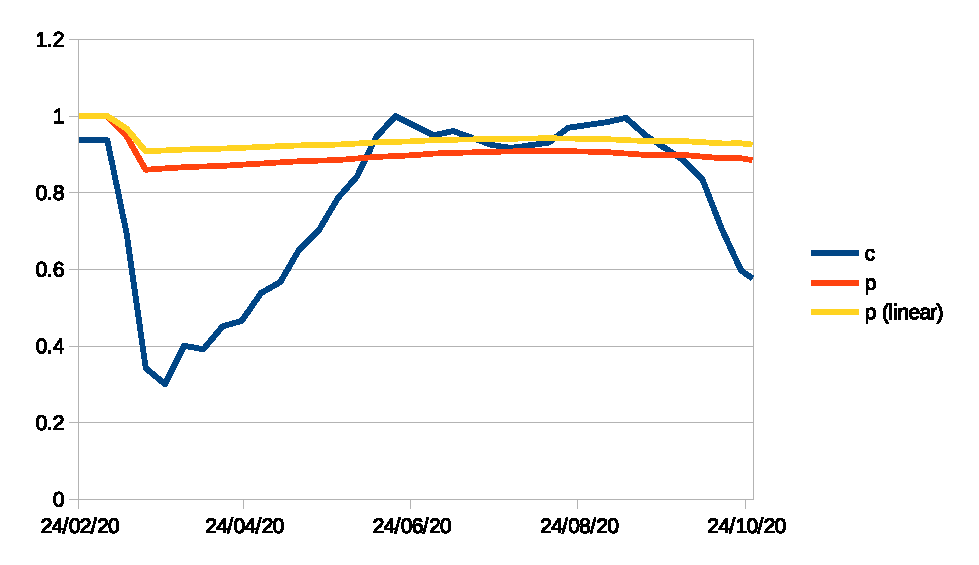
\includegraphics[scale=0.3]{cp} & 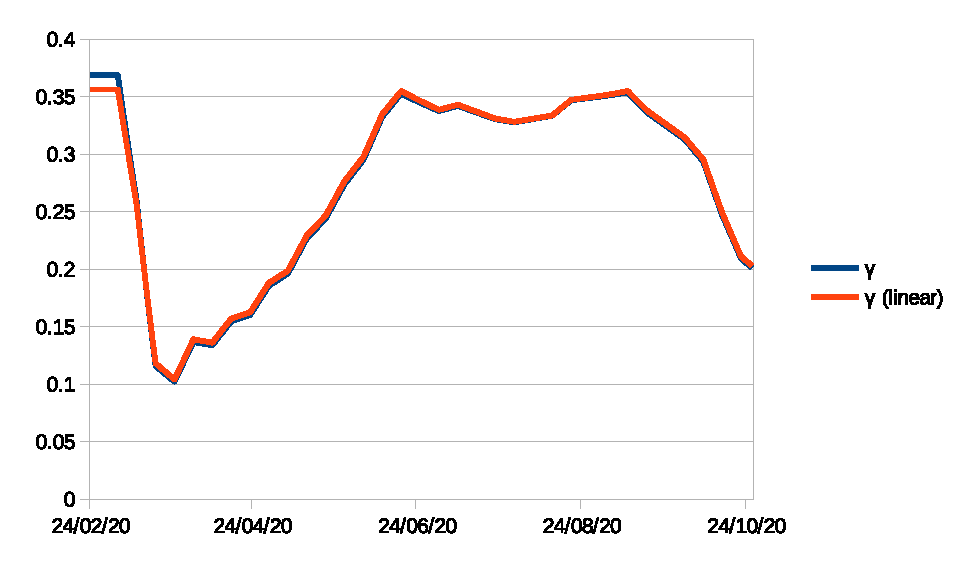
\includegraphics[scale=0.3]{gamma}\tabularnewline
\hline 
\end{tabular}

It is clear that the original and the linearized models are practically
equivalent, so we will refer only to the linear one until the end
of the paragraph.

x

x

x

y

A question arises what $I_{t}$ and $P_{t}$ should be so that $Z_{t}\rightarrow0$.

Let $U=\{E,I_{a},I_{s},I_{n}\}$ We have 
\[
\barP=\left[\begin{array}{cccc}
p^{E} & \iota & \iota & \iota\\
p^{Ea} & p^{aa} & 0 & 0\\
0 & p^{as} & p^{ss} & 0\\
p^{En} & 0 & 0 & p^{nn}
\end{array}\right]
\]
and we have 
\begin{multline*}
|\barP-\lambda I|=\left|\begin{array}{cccc}
p^{E}-\lambda & \iota & \iota & \iota\\
p^{Ea} & p^{aa}-\lambda & 0 & 0\\
0 & p^{as} & p^{ss}-\lambda & 0\\
p^{En} & 0 & 0 & p^{nn}-\lambda
\end{array}\right|\\
=(p^{E}-\lambda)\left|\begin{array}{ccc}
p^{aa}-\lambda & 0 & 0\\
p^{as} & p^{ss}-\lambda & 0\\
0 & 0 & p^{nn}-\lambda
\end{array}\right|-\iota\left|\begin{array}{ccc}
p^{Ea} & 0 & 0\\
0 & p^{ss}-\lambda & 0\\
p^{En} & 0 & p^{nn}-\lambda
\end{array}\right|\\
+\iota\left|\begin{array}{ccc}
p^{Ea} & p^{aa}-\lambda & 0\\
0 & p^{as} & 0\\
p^{En} & 0 & p^{nn}-\lambda
\end{array}\right|-\iota\left|\begin{array}{ccc}
p^{Ea} & p^{aa}-\lambda & 0\\
0 & p^{as} & p^{ss}-\lambda\\
p^{En} & 0 & 0
\end{array}\right|\\
=(p^{E}-\lambda)(p^{nn}-\lambda)(p^{aa}-\lambda)(p^{ss}-\lambda)\\
-\gamma(p^{nn}-\lambda)(p^{ss}-\lambda)+\iota(p^{nn}-\lambda)p^{Ea}p^{as}-\gamma(p^{ss}-\lambda)(p^{aa}-\lambda)
\end{multline*}
\begin{align*}
\frac{\partial f}{\partial\iota} & =-p^{Ea}(p^{nn}-\lambda)(p^{ss}-\lambda)+(p^{nn}-\lambda)p^{Ea}p^{as}-p^{En}(p^{ss}-\lambda)(p^{aa}-\lambda)
\end{align*}
\[
\frac{\partial f}{\partial p^{ss}}=(p^{E}-\lambda)(p^{nn}-\lambda)(p^{aa}-\lambda)-\gamma(p^{nn}-\lambda)-\gamma(p^{aa}-\lambda)
\]
\\
\begin{multline*}
p^{ss}'(\iota)=\frac{f_{\iota}}{f_{ss}}
\end{multline*}

\end{document}

x

x

Denote $M_{t}=\E(X_{t},Y_{t}|\G_{t-1})$ and $V_{t}=\var(X_{t},Y_{t}|\G_{t-1})$.
As, given normal approximation,we get
\begin{multline*}
\E\left[\left.{X_{t+1}\atop Y_{t+1}}\right|\G_{t}\right]=\E\left[\E\left[\left.{X_{t+1}\atop Y_{t+1}}\right|\F_{t}\right]\G_{t}\right]\\
=\E\left[\left.\left[{T_{t}\atop FT_{t}}\right]X_{t}\right|\G_{t}\right]=\left[{T_{t}\atop FT_{t}}\right]N_{t},\qquad N_{t}=\E(X_{t}|\G_{t})
\end{multline*}
and 
\begin{multline*}
V_{t+1}=\var\left(\left.\E\left[\left.{X_{t+1}\atop Y_{t+1}}\right|\F_{t}\right]\right|\G_{t}\right)+\E\left(\left.\var\left[\left.{X_{t+1}\atop Y_{t+1}}\right|\F_{t}\right]\right|\G_{t}\right)\\
=\var\left[\left.\left[{T_{t}\atop FT_{t}}\right]X_{t}\right|\G_{t}\right]+\E\left[\left.\begin{array}{cc}
\Lambda_{t} & \Lambda_{t}F^{T}\\
F\Lambda_{t} & F\Lambda_{t}F^{T}+FX_{t}
\end{array}\right|\G_{t}\right]\\
=\left[{T_{t}\atop FT_{t}}\right]W_{t}\left[{T_{t}\atop FT_{t}}\right]^{T}+\sum_{i+1}^{k}\left[\begin{array}{cc}
\Phi_{i} & \Phi_{i}F^{T}\\
F\Phi_{i} & F\Phi_{i}F^{T}
\end{array}\right]N_{t}^{i}+\left[\begin{array}{cc}
J_{t} & J_{t}F^{T}\\
FJ_{t} & FJ_{t}F^{T}+\Gamma tbdN_{t}
\end{array}\right]
\end{multline*}
where $J_{t}=\mathrm{diag}(I_{t}N_{t})$
\end{document}
